\begin{wrapfigure}{l}{25mm}
    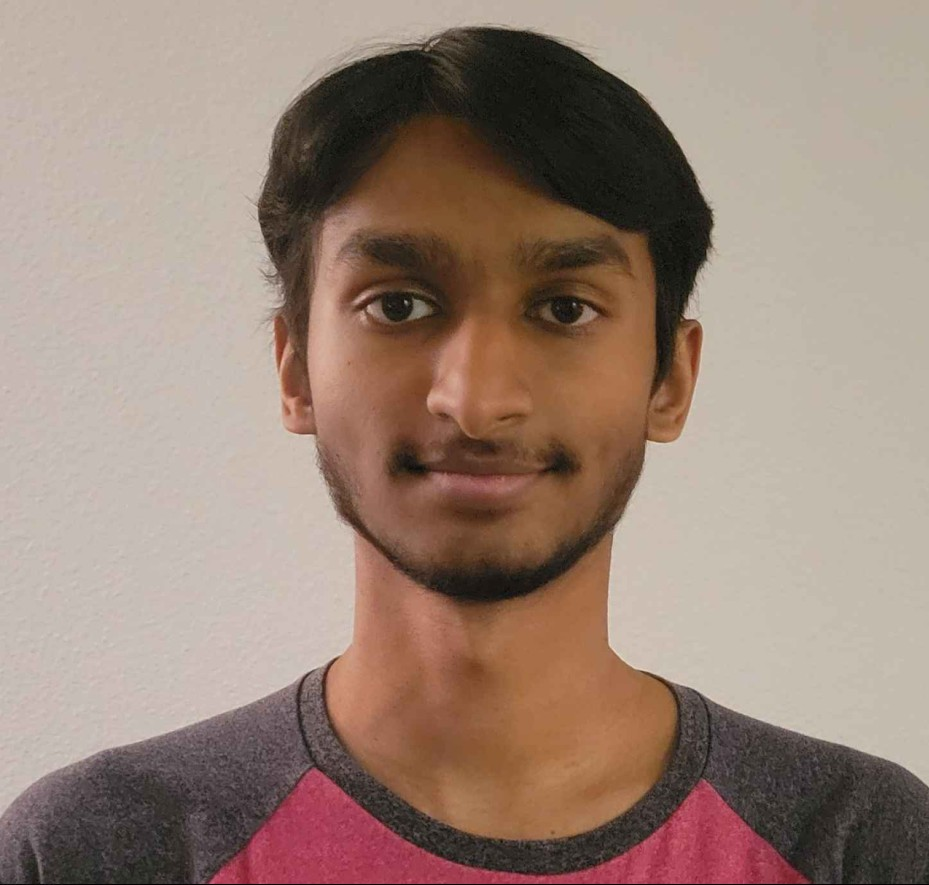
\includegraphics[width=0.95\linewidth]{figures/dibyesh_bio.jpg}
\end{wrapfigure}\par

\textbf{Dibyesh Sahoo} is a graduate student in Computer Engineering at UC San Diego, where he also earned his B.S. in Computer Engineering. His technical background includes experience with Go, Rust, Java, and C. His interests include high-performance systems, networking, and scalable infrastructure.

\begin{wrapfigure}{l}{25mm}
    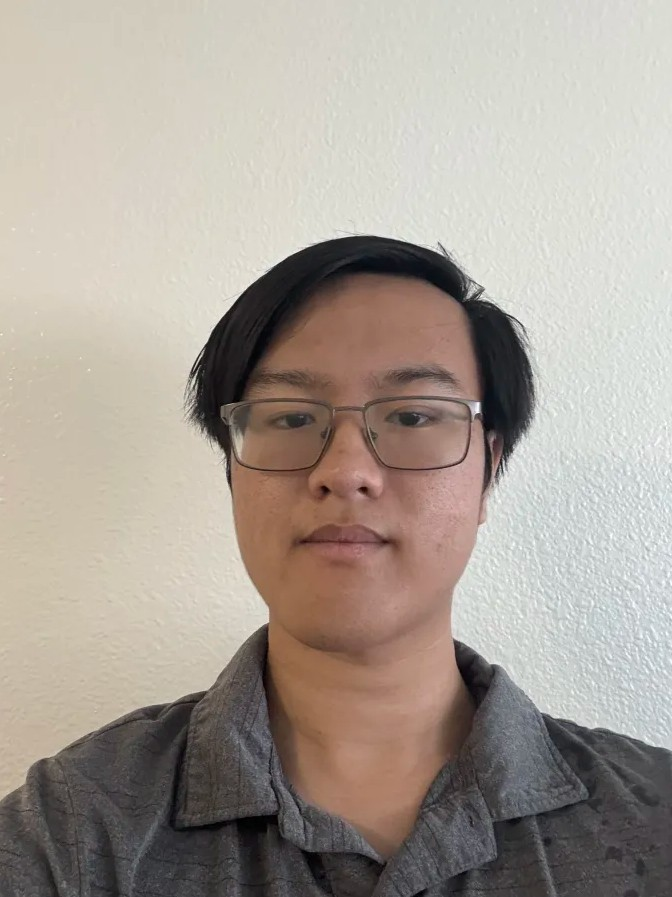
\includegraphics[width=0.95\linewidth]{figures/daniel_bio.jpg}
\end{wrapfigure}\par

\textbf{Daniel Tran} is an MS student at UCSD’s Electrical and Computer Engineering department, where he got his BS in Computer Engineering. His technical background includes experience with Verilog, Python, and Java. His interests include ML applications, network analysis, and ASIC design.


\begin{wrapfigure}{l}{25mm}
    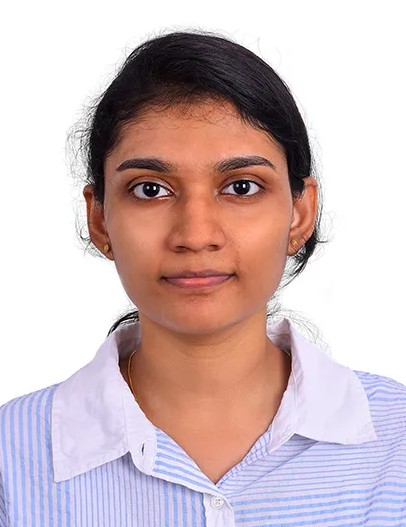
\includegraphics[width=0.95\linewidth]{figures/anjana_bio.jpg}
\end{wrapfigure}\par

\textbf{Anjana Manoj} is an MS student at UCSD’s Electrical and Computer Engineering department. She completed her Bachelor's in Electronics and Communication Engineering from the National Institute of Technology, Calicut, India. Her technical background includes experience with Verilog, Python, and C++. Her interests include ASIC design, ASIC test methodologies, and network design. 

\begin{wrapfigure}{l}{25mm}
    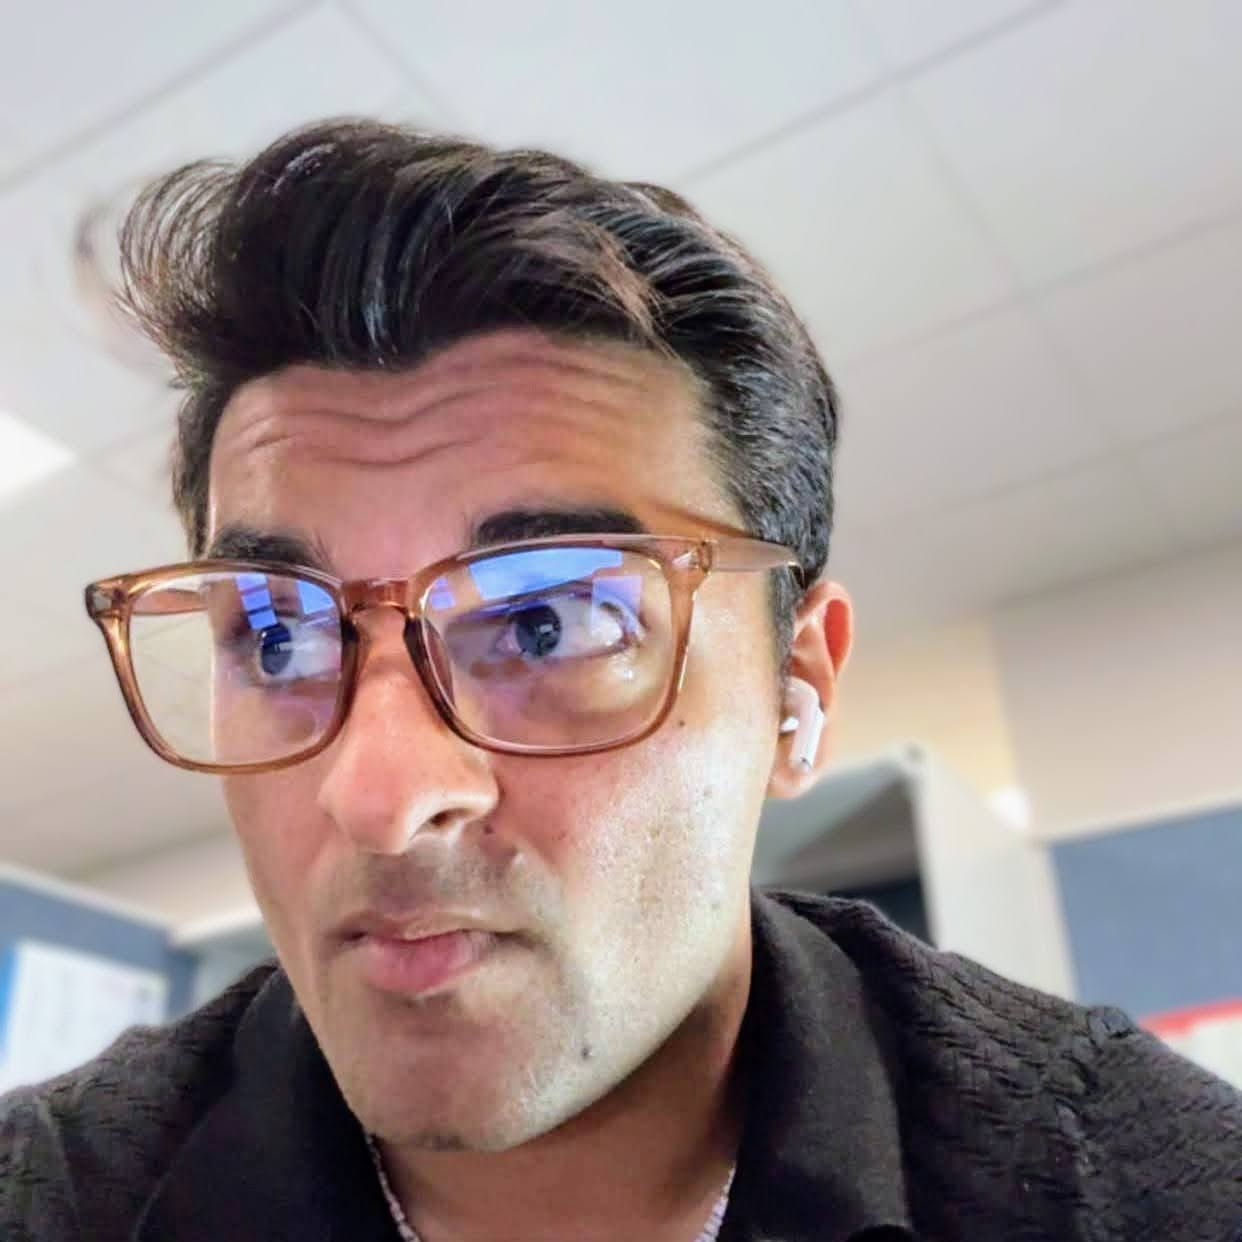
\includegraphics[width=0.95\linewidth]{figures/russ_bio.jpg}
\end{wrapfigure}\par
\textbf{Russ Sobti} is a MS student at UCSD’s Electrical and Computer Engineering department. He completed his Bachelor's in Computer Engineering from the California State University, San Luis Obispo. His technical background includes experience with Verilog, Python, and C++ as well as embedded RF systems. His interests include wireless communication systems, embedded architectures, and FPGA/ASIC design.